\normaltrue
\correctionfalse

%\UPSTIidClasse{12} % 11 sup, 12 spé
%\newcommand{\UPSTIidClasse}{12}

\exer{Mouvement R  $\star$ \label{C2:09:02}}
\setcounter{question}{0}\UPSTIcompetence[2]{C2-09}
\index{Compétence C2-09}
\index{Principe fondamental de la dynamique}
\index{PFD}
\index{Mécanisme à 1 rotation}
\ifcorrection
\else
\marginnote{\textbf{Pas de corrigé pour cet exercice.}}
\fi

\ifprof
\else
Soit le mécanisme suivant. On a $\vect{AB}=R\vect{i_1}$ avec $R=\SI{20}{mm}$. La liaison pivot est motorisée par un moteur modélisée dont l'action mécanique sur \textbf{1} est donnée par $\vect{C_m}=C_m \vect{k_0}$ avec $C_m = \SI{40}{Nm}$. La fréquence de rotation nominale est de $1\,500\; \text{tr}\,\text{min}^{-1}$. 

 La pesanteur est telle que $\vect{g}=-g\vect{j_0}$.
On note $m_1$ la masse du solide 1, $B$ son centre d'inertie et $\inertie{B}{1}=\matinertie{A_1}{A_1}{A_1}{0}{0}{0}{\bas{1}}$ avec $A_1 = 12,5\; \text{kg}\,\text{m}^2$.
 Le couple résistant dû aux frottements est supposé constant et égal à $4\, \text{N} \, \text{m}$.

(On notera $J$ le moment dynamique du solide 1 autour de l'axe $\axe{A}{k_0}$.

\begin{center}
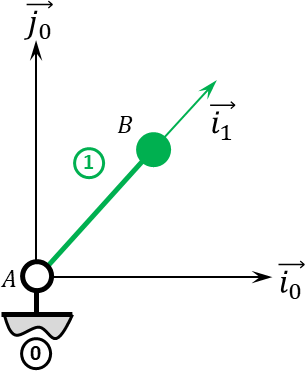
\includegraphics[width=\linewidth]{02_R_01}
\end{center}

\fi


\question{Calculer l’accélération du moteur pendant le démarrage.}
\ifprof
\else
\fi

\question{Calculer le temps mis pour atteindre la fréquence nominale.}
\ifprof
\else
\fi



\ifprof
\else
\begin{flushright}
\footnotesize{Corrigé  voir \ref{C2:09:02}.}
\end{flushright}%
\fi